%**
% \PutAt<overlay spec>[<box width>]{(<x>, <y>)}{<content>}
%
% real absolute positioning of <content> on a slide, if content is a figure,
% minipage or whatever kind of LR-box, the <box width> argument may be omitted
%
%
% implementation notes: 
%   - based on   \usepackage[absolute,overlay]{textpos}
%   - NOT combinable with any beamer feature that is based on pgfpages
%     (such as dual-screen support, built-in 2up handouts, etc.), as textpos 
%     and pgfpates interfere at the shippout-level.
%

  \newcommand<>{\PutAt}[3][0pt]{%
    {\only#4{\begin{textblock*}{#1}#2%
      #3
    \end{textblock*}}}%
  }

%**
% \ShowPutAtGrid
%
% draws a helpful grid on the current slide to figure <x> and <y> parameters for \PutAt
% 
  \newcommand{\ShowPutAtGrid}{
    \begin{textblock*}{128mm}(0cm,0cm)
    \tikz[color=red!20!white]\draw[very thin, step=5mm] (0mm,0mm) grid (130mm,100mm);
    \end{textblock*}
    \begin{textblock*}{128mm}(0cm,0cm)
    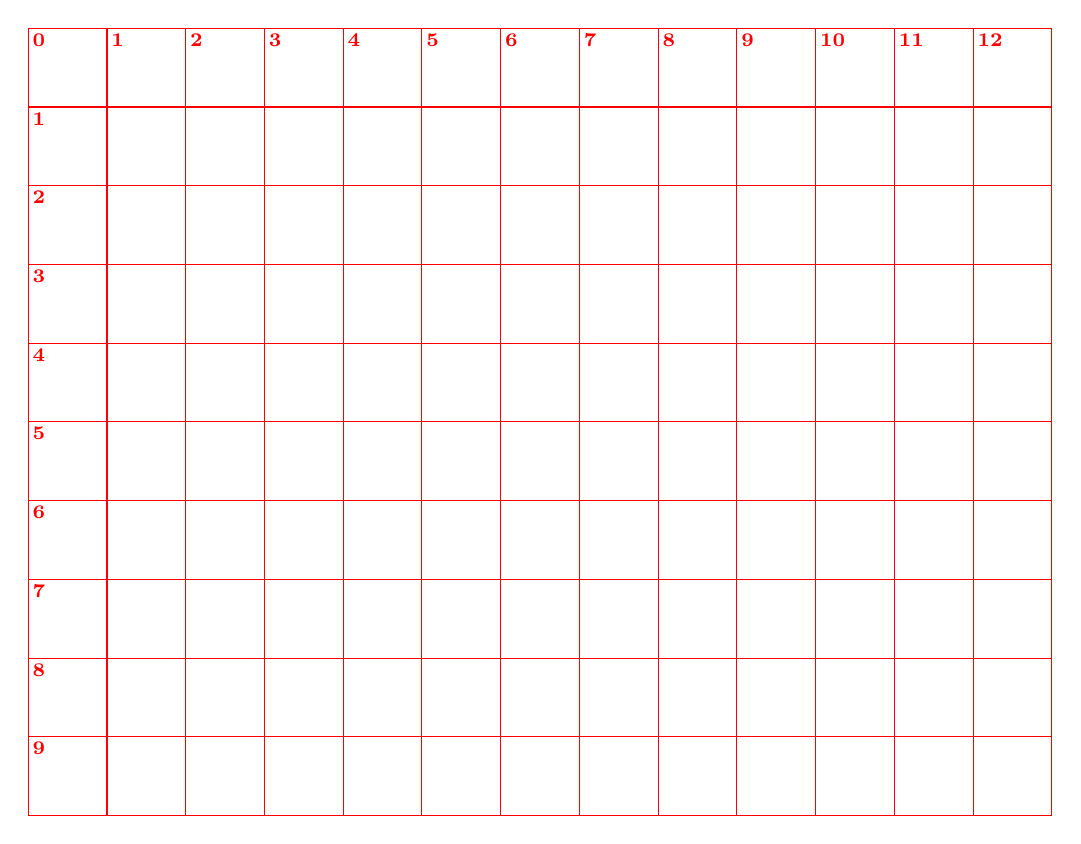
\begin{tikzpicture}[color=red]
      \draw[step=1cm] (0,0mm) grid (130mm,100mm);   
      \foreach \n in {0,...,12}
        \draw[xshift=.5mm,yshift=-1.5mm, inner sep=0pt, anchor=west] (\n,10) node {\scriptsize{\textbf{\n}}};
      \foreach \n in {1,...,9}
        \draw[xshift=.5mm,yshift=-1.5mm, inner sep=0pt, anchor=west] (0,10-\n) node {\scriptsize{\textbf{\n}}};
    \end{tikzpicture}
    \end{textblock*}
  }


%**
% \NormalBox<overlay spec>[tikz picture/node options]{<content>}
%
% draws content boxed in a nice box
% 
\newcommand<>{\NormalBox}[2][]{%
  \only#3{\tikz[#1, every node/.style={shape=rectangle,draw,fill=white, drop shadow, #1}]\node []{#2};}
}
%**
% \OrangeBox<overlay spec>[tikz picture/node options]{<content>}
%
% draws content boxed in an orange call-out box
% 
\newcommand<>{\OrangeBox}[2][]{%
  \onslide#3{\NormalBox[fill=orange!30,draw=black!30,rounded corners=4pt,#1]{#2}}%
}
%**
% \NoBox<overlay spec>[tikz picture/node options]{<content>}
%
% draws content boxed in a nice box
% 
\newcommand<>{\NoBox}[2][]{%
  \only#3{\tikz[#1, every node/.style={shape=rectangle, #1}]\node []{#2};}
}
